% ======================= Pre-Amble =========================

\documentclass[11pt, oneside]{article}   	% use "amsart" instead of "article" for AMSLaTeX format 
                     						%imports package {article} and specify option(s) [11pt, oneside]
\usepackage{geometry}                		% See geometry.pdf to learn the layout options. There are lots.                                        

\geometry{letterpaper}                   		% ... or a4paper or a5paper or ... 
%\geometry{landscape}                		% Activate for rotated page geometry

\usepackage[parfill]{parskip}    		        % Activate to begin paragraphs with an empty line rather than an indent

\usepackage[hidelinks]{hyperref}                % Allows for clickable references

%American Mathematics Society packages
\usepackage{amsmath}	   %math
\usepackage{amssymb}       %symbols
\usepackage{amsthm}          %theorems

%Graphics
\usepackage{graphicx}
\usepackage[usenames, dvipsnames]{color}     % font colour:    \textcolor{<colour>}{text}
      									%highlight text:  \colorbox{<color>}{text}
									
									%list of colours: https://www.sharelatex.com/learn/Using_colours_in_LaTeX

%Images		                
\graphicspath{ {images/} }                          %directory that your images are located in within your current directory
	

%Footnote Spacing
\setlength{\footnotesep}{0.4cm}                  %specify spacing b/w footnotes
\setlength{\skip\footins}{0.6cm}                    % space b/w footnotes and textbody

%Table
\usepackage[none]{hyphenat}                    % Stops breaking-up words in a table (i.e. no hyphens)
                                                               

\usepackage{array}   
\newcolumntype{x}[1]{>{\centering\let\newline\\\arraybackslash\hspace{0pt}}p{#1}}       %center fixed column width: x{<len>}                      
\newcolumntype{$}{>{\global\let\currentrowstyle\relax}}                                                   % let us apply things (e.g. bold/italicize) to entire row            
\newcolumntype{^}{>{\currentrowstyle}}
\newcommand{\rowstyle}[1]{\gdef\currentrowstyle{#1} #1\ignorespaces}

%Bibliography
\usepackage[numbers,sort&compress]{natbib}   %for multiple references: sorts  (i.e. [1,2] NOT [2, 1] )
                                           				  %                                     compresses (i.e. [1-3] )
\usepackage[nottoc]{tocbibind}                            %add bibliography to table of contents

%Diagrams
\usepackage[latin1]{inputenc}
\usepackage{tikz}
\usetikzlibrary{shapes,arrows}
	

\usepackage{dirtytalk}    %quotations: use \say  

\usepackage{caption}
\captionsetup[figure]{labelfont=bf}    %make figure labels boldface
\captionsetup[table]{labelfont=bf}     %make table labels boldface

%Bullets
\usepackage{enumerate}     %specify type of enumeration: \being{enumerate}[<type of enumeration>]

%QED
\newcommand*{\QEDA}{\hfill\ensuremath{\blacksquare}}         %make qed filled square:    \QEDA
%\newcommand*{\QEDB}{\hfill\ensuremath{\square}}               %make qed empty square: \QEDB 

%Header and Footer
\usepackage{fancyhdr}
\usepackage{lastpage}      %ensures you can reference LastPage (i.e. Page 2 of 10)

%Diagrams
\usepackage[latin1]{inputenc}
\usepackage{tikz}
\usetikzlibrary{shapes,arrows}

%\usepackage{tikz}
\usepackage{tikz,fullpage}
\usetikzlibrary{arrows,%
                petri,%
                topaths}%
\usepackage{tkz-berge}
\usepackage[position=top]{subfig}


%=========== Header & Footer =========================

\pagestyle{fancy}
\lhead{Stephanie Knill} 		% controls the left corner of the header
\chead{} 					% controls the center of the header
\rhead{} 					% controls the right corner of the header
\lfoot{} 					% controls the left corner of the footer
\cfoot{Page~\thepage\ of \pageref{LastPage}} 				% controls the center of the footer
												%Page~\thepage\  if just want Page x
\rfoot{}			 		% controls the right corner of the footer
\renewcommand{\headrulewidth}{0.4pt}
\renewcommand{\footrulewidth}{0.4pt}

\setlength{\headsep}{0.3in}		%space b/w page header and body

% ======================== Document ======================
\begin{document}

\title{MATH 442 --- Assignment 2 \\
\line(1,0){360} \\              %(slope x, y){length of line}
}
\author{
Stephanie Knill \\
54882113 \\
Due: January 14, 2015}

\date{}                   % Activate:  display a given date (e.g. {August 4} ) or no date (empty {} )
                                    %No activate: display current date
\maketitle


\thispagestyle{empty}                   %Remove header from this (first) page. Change empty -> plain to keep numbering

% ================= Questions ================

\section*{Question 7}

In order to have an Euler cycle---a cycle utilizing each edge of a graph exactly once---in a graph, all vertices must be of even degree. In the case of the town K{\"o}onigsburg, we can express it as a graph where each land mass is represented by a vertex and each bridge by an edge (Figure~\ref{original}).

\begin{figure}[h]
%Latex Documentation: http://www.texample.net/tikz/examples/tkz-berge/

\centering
%\subfloat[]{                %use to number it (a)
\begin{tikzpicture}[scale=0.75,transform shape]
  \Vertex[x=0,y=0]{A}
  \Vertex[x=3,y=2]{B}
  \Vertex[x=6,y=0]{C}
  \Vertex[x=3,y=-2]{D}

  \tikzstyle{LabelStyle}=[fill=white,sloped]
  %Edges bend left
  \tikzstyle{EdgeStyle}=[bend left]
      \Edge(A)(B)				%\Edge[label=$120$](A)(B)  %if want to label the edge
      \Edge(A)(D)
      \Edge(B)(C)
  %Edges bend right
  \tikzstyle{EdgeStyle}=[bend right]
      \Edge(A)(B)
      \Edge(A)(D)
      \Edge(D)(C)
  %Edges straight
  \tikzstyle{EdgeStyle}=[]
      \Edge(A)(C)
    
\end{tikzpicture}
%}
\caption{Graph of K{\"o}onigsburg. Landmasses are represented by vertices and bridges by edges.}
\label{original}
\end{figure}

Since all vertices are of odd degree ($deg(A) = 5, deg(B) = deg(C) = deg(D) = 3$), we need to remove at least \textbf{two} edges between two different pairs of odd degree vertices. Without loss of generality, let us remove the edges between vertices $A$ and $B$ and vertices $C$ and $D$. This leaves us with vertices of $deg(A) = 4, deg(B) = deg(C) = deg(D) = 2$. Since all vertices are now even, an Euler cycle is feasible. An example Euler tour of the form $A \rightarrow B \rightarrow C \rightarrow A \rightarrow D \rightarrow A$ is shown in Figure~\ref{removed}.


\begin{figure}[h]
\centering
%\subfloat[]{                %use to number it (a)
\begin{tikzpicture}[scale=0.75,transform shape]
  \Vertex[x=0,y=0]{A}
  \Vertex[x=3,y=2]{B}
  \Vertex[x=6,y=0]{C}
  \Vertex[x=3,y=-2]{D}

  \tikzstyle{LabelStyle}=[fill=white,sloped]
  %Edges bend left
  \tikzstyle{EdgeStyle}=[post, bend left]
      \Edge(A)(B)				%\Edge[label=$120$](A)(B)  %if want to label the edge
      \Edge(A)(D)
      \Edge(B)(C)
  %Edges bend right
  \tikzstyle{EdgeStyle}=[pre, bend right]
      \Edge(A)(D)
  %Edges straight
  \tikzstyle{EdgeStyle}=[pre]
    \Edge(A)(C)
\end{tikzpicture}
%}

\caption{Directed graph of K{\"o}onigsburg with two bridges removed.}
\label{removed}
\end{figure}


\cleardoublepage
\section*{Question 8}

In order to construct an Euler path in the town of K{\"o}onigsburg, we must have only 2 odd degree vertices. At an even degree vertex, you go both in \textit{and} out of the vertex. Whereas at an odd vertex, you either go in \textit{or} out of the vertex. Therefore with 2 odd degree vertices, one will be the starting vertex and the other will be the terminal vertex. Since we have 4 vertices of odd degree, we can without loss of generality demolish any one of the bridges. For example, let us demolish the bridge connecting vertex $A$ to vertex $C$. This leaves us with vertices of $deg(A) = 4, deg(B) = deg(C) 3, deg(D) = 2$. An example Euler tour of the form $B \rightarrow C \rightarrow D \rightarrow A \rightarrow B \rightarrow A \rightarrow D$ is shown in Figure~\ref{euler path}. Note how we start and end at the two odd degree vertices $B$ and $D$.

\begin{figure}[h]
\centering
%\subfloat[]{                %use to number it (a)
\begin{tikzpicture}[scale=0.75,transform shape]
  \Vertex[x=0,y=0]{A}
  \Vertex[x=3,y=2]{B}
  \Vertex[x=6,y=0]{C}
  \Vertex[x=3,y=-2]{D}

  \tikzstyle{LabelStyle}=[fill=white,sloped]
  %Edges bend left
  \tikzstyle{EdgeStyle}=[post, bend left]
      \Edge(A)(B)				%\Edge[label=$120$](A)(B)  %if want to label the edge
      \Edge(A)(D)
      \Edge(B)(C)
  %Edges bend right
  \tikzstyle{EdgeStyle}=[pre, bend right]
      \Edge(A)(B)
      \Edge(A)(D)
      \Edge(D)(C)
      

\end{tikzpicture}
%}

\caption{Directed graph of K{\"o}onigsburg with one bridge removed.}
\label{euler path}
\end{figure}


\section*{Question 9}

On a 3 x 4 chessboard, it is possible as a knight to visit each of the squares exactly once; however, you will not be able to start and finish at the same place. An example Euler walk is depicted in Table~\ref{euler walk}.

\begin{table}[h]                                          %optional argument: place figure/table here (h), top (t), page of floats (p)
\begin{center}
\begin{tabular}{| c | c | c | c |}            %{$p{1.2cm} | ^ x{2.9cm} || ^c |^c}                     %use x{<len>} to centre a column of length <len> 
    
    \hline
    10 & 7 & 2 & 5 \\
    \hline
     1 & 4 & 9 & 12 \\
     \hline
     8 & 11 & 6 & 3\\
     \hline

\end{tabular}
\end{center}
\caption{Euler walk for a knight on a 3 x 4 chessboard.}
\label{euler walk}
\end{table}


Here, each number $i = 1, 2, \ldots , 12$ represents the order in which a square is visited. This means we start at $i=1$ and end at $i=12$.

According to the nature governing how a knight moves, if a knight starts on a \textit{white} square it can only move to a \textit{black} square; conversely, if a knight starts on a \textit{black} square it can only move to a \textit{white} square. In a board of odd number of squares, there is an unequal number of black and white squares. Therefore if a knight were to start on a white square, it will end on a  black square; likewise, if a knight were to start on a black square, it will end on a white square. Thus, a knight's tour on an odd number of squares board cannot be conducted such that the knight starts and ends on the same square.

\cleardoublepage
\section*{Question 10}

The given parse tree can be alternatively expressed as

$$((4t-5w)(x+y))*((y+w+z)+(2x+1+y)/(3+5w^2))$$



\section*{Question 11}

\textit{\textbf{Conjecture:} The game of Sprouts with $n$ vertices must terminate after at most $3n-1$ moves.}
%\vspace{0.1cm}

\textbf{Proof by Construction}

Since no vertex can have more than 3 edges coming out of it, our initial isolated graph of $n$ vertices has $3n$ degrees available to \say{play} with. If we are to draw an edge, we will have one less degree available, or $3n-1$ degrees. Thus with each successive edge drawn, we will have $3n-1, 3n-2, 3n-3, \ldots$ degrees available.

Since the loser is the first player who cannot make a move, we have 2 possible termination cases: 1) one vertex has degree less than three; or 2) two or more vertices have degree less than three but joining them would cross an edge. The first case has the maximum number of moves in a given game, so we will only consider this case. In this scenario, we only have 1 degree available after the last move. Hence the set of degrees available after each move is given by $S = {3n-1, 3n-2, \ldots , 1}$. To find the total number of moves in this maximal moves case, we need only take the cardinality of the set. Because $|S| = 3n-1$, it follows that the game of Sprouts with $n$ vertices must terminate after at most $3n-1$ moves. \QEDA 

Thanks to a collaborative effort\footnote{Or to put it more accurately, a \say{sprouts-off}.} between Ian Yihang Zhu, Thomas Roehrl and myself, a game of sprouts with 3 vertices that terminated after 6 moves was finally produced:

\vspace{6cm}

Although the graph could have been visually simplified, it was deemed that the game in all of its original, swirly glory must be preserved.



\cleardoublepage
\section*{Question 12}

\textit{\textbf{Claim:} In a party of 6 people it is true there exists 4 people who all do know each other or there exists 4 people who all do not know each other.}
\vspace{0.1cm}

Let a solid edge between two vertices represent if the people know each other and a dotted edge between two vertices represent if the people do not know each other. For this claim to hold true, there must always exist a subgraph that is a complete graph $K_4$ compose entirely of solid or dotted edges. In the following counterexample (Figure~\ref{party of 6})
%\vspace{7cm}

\begin{figure}[h]
\centering
%\subfloat[]{                %use to number it (a)
\begin{tikzpicture}[scale=0.75,transform shape]
  \Vertex[x=0,y=0]{A}
  \Vertex[x=3,y=2]{B}
  \Vertex[x=6, y=2]{C}
  \Vertex[x=9,y=0]{D}
  \Vertex[x=6,y=-2]{E}
  \Vertex[x=3,y=-2]{F}

  \tikzstyle{LabelStyle}=[fill=white,sloped]
  %Edges bend left
  \tikzstyle{EdgeStyle}=[bend left]


  %Edges bend right
  \tikzstyle{EdgeStyle}=[dashed, bend right]
  %Edges straight solid
  \tikzstyle{EdgeStyle}=[]
      \Edge(B)(F)
      \Edge(B)(C)
      \Edge(E)(F)
      \Edge(C)(E)
      \Edge(B)(E)
      \Edge(A)(B)	
      \Edge(A)(F)
      \Edge(C)(D)
      \Edge(D)(E)
      \Edge(A)(D)

   %Edges straight dotted
   \tikzstyle{EdgeStyle}=[dashed]
      \Edge(C)(F)
      \Edge(E)(F)	
      \Edge(B)(D)
      \Edge(A)(C)
      \Edge(A)(E)
      \Edge(D)(F)

\end{tikzpicture}
%}

\caption{Graph of party of 6 people, where each person is represented by a node. Relationship between two people is indicated by an edge: solid line if they know each other or dashed line if they do not.}
\label{party of 6}
\end{figure}

we can see that no such subgraph $K_4$ exists, thereby disproving the claim.







\end{document} 